\documentclass[11pt]{beamer}
\usetheme{Pittsburgh}
\usepackage[utf8]{inputenc}
\usepackage[portuguese]{babel}
\usepackage[T1]{fontenc}
\usepackage{amsmath}
\usepackage{amsfonts}
\usepackage{amssymb}
\usepackage{graphicx}
\usepackage{hyperref}
\author{Sara Mortara, Andrea Sanchez-Tapia \& Diogo Rocha}
\title{um apanhado de dicas de como usar Git (bem, ou um pouco melhor)}
\newcommand{\code}{\texttt}
%\setbeamercovered{transparent} 
%\setbeamertemplate{navigation symbols}{} 
%\logo{} 
%\institute{} 
%\date{} 
%\subject{} 
\begin{document}

\begin{frame}
\titlepage
\end{frame}

%\begin{frame}
%\tableofcontents
%\end{frame}

\begin{frame}{o que é 
\includegraphics[scale=0.2]{logo-git.png}}

sistema de controle de versão \textbf{livre} e de \textbf{código aberto}

\begin{itemize}
\item pegada
\item alta performance
\item múltiplos fluxos de trabalho
\item \textit{branching} & \textit{merging}
\item distribuição - \textit{clone}
\item área intermediária - \textit{staging area}
\end{itemize}

\end{frame}

\begin{frame}{o que é 
\includegraphics[scale=0.2]{github.jpeg}}

serviço de hospedagem na internet para controle de versão e colaboração usando \textbf{git}

\begin{itemize}

\end{itemize}

\end{frame}


\begin{frame}{por onde começar}

\begin{itemize}
\item guia básico de \textbf{Git} no \textbf{GitHub}:

\subitem \href{https://guides.github.com/activities/hello-world/}{https://guides.github.com/activities/hello-world/}

\item como usar o \textbf{Git} no \textbf{RStudio}:

\subitem \href{https://pagepiccinini.com/r-course/lesson-0-introduction-and-set-up/}{https://pagepiccinini.com/r-course/lesson-0-introduction-and-set-up/}

\end{itemize}

\end{frame}

\begin{frame}{fluxo básico de trabalho}
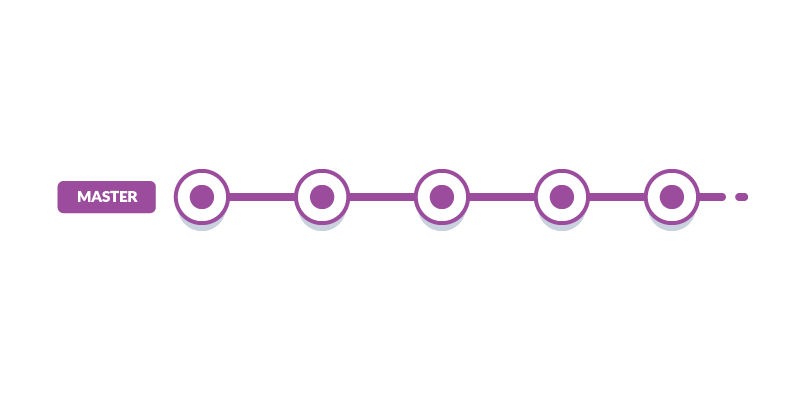
\includegraphics[scale=.4]{basic.png}
\end{frame}

\begin{frame}{fluxo de trabalho \textit{feature}}
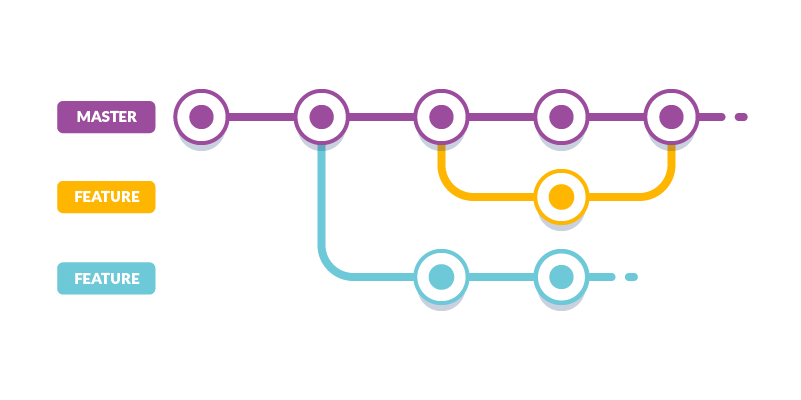
\includegraphics[scale=.4]{feature-branch.png}
\end{frame}


\begin{frame}{em outras palavras}
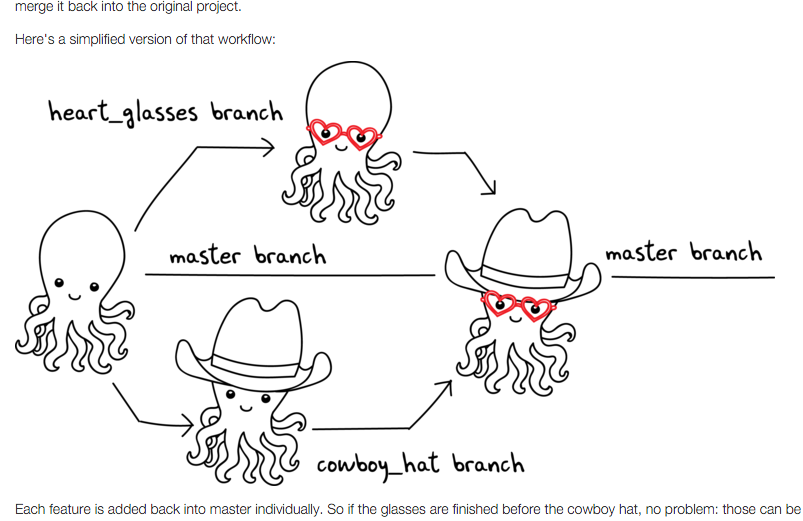
\includegraphics[scale=.4]{jennifer_gilbert.png}
\end{frame}


\begin{frame}{fluxo de trabalho \textit{gitflow}}
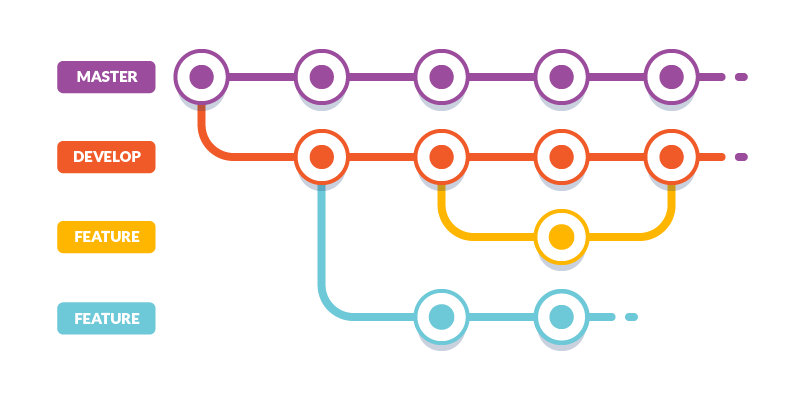
\includegraphics[scale=.4]{gitflow.png}
\end{frame}

\begin{frame}{o exemplo do modleR}

\href{https://github.com/Model-R/modelr_pkg}{https://github.com/Model-R/modelr\_pkg}


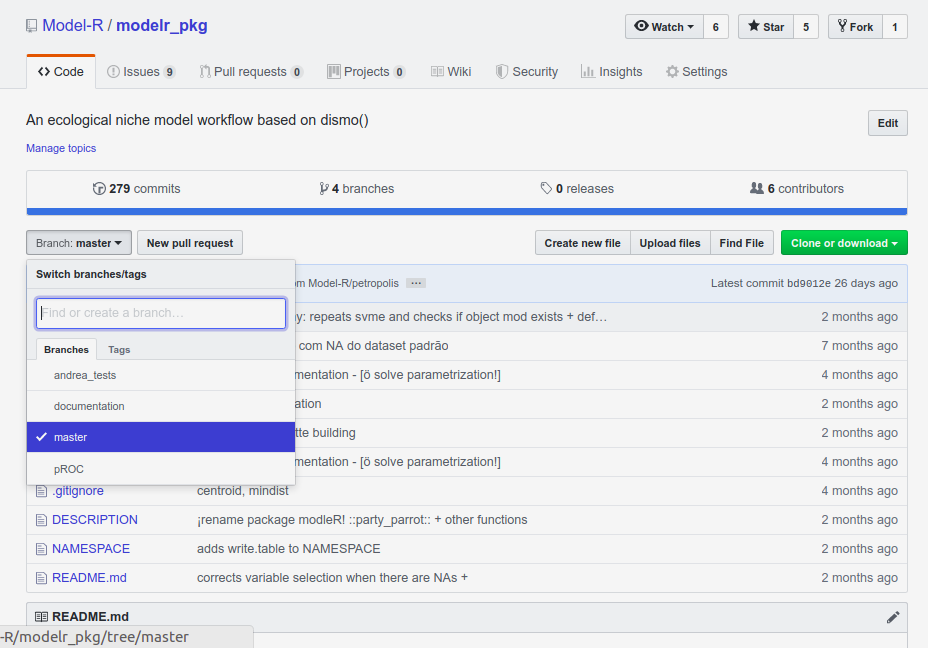
\includegraphics[scale=.3]{print1.png}

\end{frame}


\begin{frame}{fluxo de trabalho do pacote modleR}
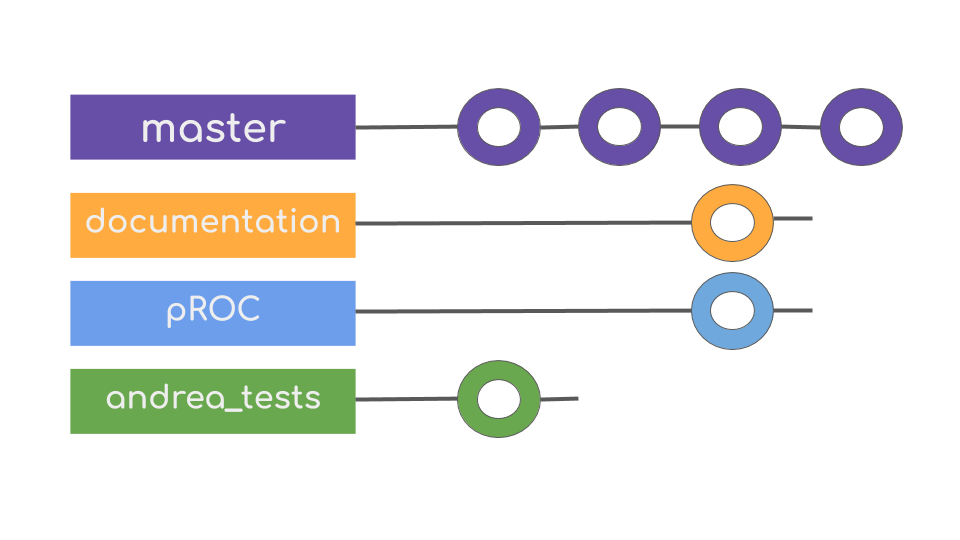
\includegraphics[scale=.3]{git.png}
\end{frame}

\begin{frame}{comandos básicos}

%\begin{itemize}
     \begin{block}{Para clonar um repositório já existente: }
      \code{git clone https://github.com/Model-R/modelr\_pkg.git}
      \end{block}
%\item 
   \begin{block}{Para criar um repositório git localmente: }
         \code{git init}
        \end{block}
%\code {git init }

%\end{itemize}


\end{frame}


\begin{frame}{os meus \textbf{quatro} comandos básicos}

     \begin{block}{1. Para atualizar o repo localmente: }
      \code{git pull origin master}
      \end{block}

   \begin{block}{2. Para adicionar um arquivo com mudanças:}
         \code{git add filename}
        \end{block}
        
          \begin{block}{3. O \textit{commit}:}
         \code{git commit -m "uma mensagem informativa para você e coleguinhxs"}
        \end{block}

     \begin{block}{4. Enviando para o repositório:}
         \code{git push origin master}
        \end{block}


\end{frame}

\begin{frame}{boas práticas}

\begin{enumerate}

\pause \item descrever no \textbf{\textit{commit}} a mudança

\pause \item trabalhar uma tarefa em cada \textbf{\textit{branch}}

\pause \item \code{.gitignore}

\pause \item usar modo \textit{\textbf{diff}} para acompanhar mudanças no código

\pause \item reportar erros no código em \textbf{\textit{issues}}

\end{enumerate}

\end{frame}

\end{document}